\documentclass{../khlslides}


\title[Fundamenten]{Conditionals}
\author{Fr\'ed\'eric Vogels}


\pgfkeys{/tikz/flowchart/node/.style={rectangle,fill=blue,opacity=0.5,text opacity=1,drop shadow,inner sep=2mm}}
\pgfkeys{/tikz/flowchart/arrow/.style={-latex,flowchart/arrowline}}
\pgfkeys{/tikz/flowchart/arrowline/.style={thick}}


\newcommand{\lcurly}{{\tt{\char '173}}}
\newcommand{\link}[2]{\href{#1}{\beamergotobutton{#2}}}
\newcommand{\PLACEHOLDER}[1]{\ensuremath{\langle}\textrm{\textit{#1}\ensuremath{\rangle}}}


\pgfkeys{
  /wof/sequence point/.cd,
  placement/.initial=above,
  /wof/sequence link/.cd,
  label/.initial={},
  /wof/round/.cd,
  name prefix/.initial=,
  /tikz/.cd,
  sequence point/.style={blue!50,thick,fill=white},
  sequence point label/.style={font=\tiny,black},
  sequence link/.style={blue!50,thick},
  active/.style={fill=red,thick,red}
}
\newcommand{\seqpoint}[3][]{{
  \pgfkeys{/wof/sequence point/.cd,#1}
  \pgfkeys{/wof/sequence point/placement/.get=\placement}
  \pgfkeys{/wof/round/name prefix/.get=\prefix}
  \draw[sequence point] (\prefix\space#2) circle (.05)
                        node[sequence point label,\placement] {#3};
}}
\newcommand{\seqlink}[3][]{{
  \pgfkeys{/wof/sequence link/.cd,#1}
  \pgfkeys{/wof/sequence link/label/.get=\seqlinklabel}
  \pgfkeys{/wof/round/name prefix/.get=\prefix}
  \draw[sequence link] (\prefix\space#2) -- (\prefix\space#3) node[midway,sloped,yshift=1mm,font=\tiny,black] {\seqlinklabel};
}}

\newcommand{\singleround}[1][]{{
  \pgfkeys{/wof/round/.cd,#1}
  \pgfkeys{/wof/round/name prefix/.get=\prefix}
  \def\COORD (##1) at ##2;{\coordinate (\prefix\space##1) at ##2;}

  \COORD (init) at (0,0);
  \COORD (turn wheel) at ($ (\prefix\space init) + (1,2) $);
  \COORD (bankruptcy lose money) at ($ (\prefix\space turn wheel) + (1,1.5) $);
  \COORD (bankruptcy next player) at ($ (\prefix\space bankruptcy lose money) + (2,0) $);
  \COORD (pass) at ($ (\prefix\space turn wheel) + (3,0.5) $);
  \COORD (joker) at ($ (\prefix\space turn wheel) + (3,-0.5) $);
  \COORD (consonant) at ($ (\prefix\space turn wheel) + (1,-2) $);
  \COORD (show consonant) at ($ (\prefix\space consonant) + (1,0) $);
  \COORD (gain) at ($ (\prefix\space show consonant) + (1,0.5) $);
  \COORD (no consonants) at ($ (\prefix\space show consonant) + (1,-0.5) $);
  \COORD (end consonants) at ($ (\prefix\space show consonant) + (2,0) $);
  \COORD (vowel) at ($ (\prefix\space init) + (1,-2) $);
  \COORD (buy vowel) at ($ (\prefix\space vowel) + (1.5,0) $);
  \COORD (show vowels) at ($ (\prefix\space buy vowel) + (1.5,0) $);
  \COORD (no vowels) at ($ (\prefix\space show vowels) + (1,.5) $);
  \COORD (end vowels) at ($ (\prefix\space show vowels) + (2,0) $);
  \COORD (exit) at ($ (\prefix\space init) + (8,0) $);

  \seqlink[label=rad]{init}{turn wheel}
  \seqlink[label=bankroet]{turn wheel}{bankruptcy lose money}
  \seqlink{bankruptcy lose money}{bankruptcy next player}
  \seqlink[label=verlies beurt]{turn wheel}{pass}
  \seqlink[label=joker]{turn wheel}{joker}
  \seqlink[label=else]{turn wheel}{consonant}
  \seqlink{consonant}{show consonant}
  \seqlink[label=0]{show consonant}{no consonants}
  \seqlink[label=1+]{show consonant}{gain}
  \seqlink{gain}{end consonants}
  \seqlink{no consonants}{end consonants}
  \seqlink{end consonants}{exit}
  \seqlink{joker}{exit}
  \seqlink{pass}{exit}
  \seqlink{bankruptcy next player}{exit}
  \seqlink[label=klinker]{init}{vowel}
  \seqlink{vowel}{buy vowel}
  \seqlink{buy vowel}{show vowels}
  \seqlink[label=0]{show vowels}{no vowels}
  \seqlink{no vowels}{end vowels}
  \seqlink[label=1+]{show vowels}{end vowels}
  \seqlink{end vowels}{exit}

  \seqpoint[placement=above left]{init}{rad/klinker}
  \seqpoint[placement=left]{turn wheel}{draai rad}
  \seqpoint{bankruptcy lose money}{score = 0}
  \seqpoint{bankruptcy next player}{huidigeSpeler++}
  \seqpoint{pass}{huidigeSpeler++}
  \seqpoint{joker}{jokers++}
  \seqpoint[placement=below]{consonant}{gok medeklinker}
  \seqpoint{show consonant}{toon}
  \seqpoint{gain}{score += bedrag * k}
  \seqpoint[placement=below]{no consonants}{huidigeSpeler++}
  \seqpoint{end consonants}{}
  \seqpoint[placement=below]{vowel}{gok klinker}
  \seqpoint[placement=below]{buy vowel}{score -= 50}
  \seqpoint[placement=below]{show vowels}{toon}
  \seqpoint{no vowels}{huidigeSpeler++}
  \seqpoint{end vowels}{}
  \seqpoint{exit}{}
}}


\begin{document}

\begin{frame}
  \titlepage
\end{frame}

\begin{frame}
  \frametitle{Basiselementen Algoritmes}
  \begin{center}
    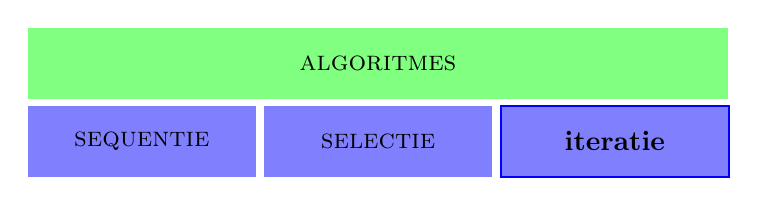
\begin{tikzpicture}[building block/.style={minimum width=2.9cm,minimum height=.9cm,fill=blue!50,font=\sc},
                        algorithm/.style={minimum width=8.9cm,minimum height=.9cm,fill=green!50,font=\sc}]
      \node[building block,anchor=south west] at (0,0) { sequentie };
      \node[building block,anchor=south west] at (3,0) { selectie };
      \node[building block,anchor=south west,draw=blue,thick] at (6,0) { \bfseries iteratie };
      \node[algorithm,anchor=south west] at (0,1) { algoritmes };
    \end{tikzpicture}
  \end{center}
\end{frame}

% \begin{frame}
  \frametitle{Rad van Fortuin}

  \begin{center}
    \begin{tikzpicture}
      \path[use as bounding box] (0,-2) rectangle (8,4);

      \coordinate (init) at (0,0);
      \coordinate (turn wheel) at ($ (init) + (1,2) $);
      \coordinate (bankruptcy lose money) at ($ (turn wheel) + (1,1.5) $);
      \coordinate (bankruptcy next player) at ($ (bankruptcy lose money) + (2,0) $);
      \coordinate (pass) at ($ (turn wheel) + (3,0.5) $);
      \coordinate (joker) at ($ (turn wheel) + (3,-0.5) $);
      \coordinate (consonant) at ($ (turn wheel) + (1,-2) $);
      \coordinate (show consonant) at ($ (consonant) + (1,0) $);
      \coordinate (gain) at ($ (show consonant) + (1,0.5) $);
      \coordinate (no consonants) at ($ (show consonant) + (1,-0.5) $);
      \coordinate (end consonants) at ($ (show consonant) + (2,0) $);
      \coordinate (vowel) at ($ (init) + (1,-2) $);
      \coordinate (buy vowel) at ($ (vowel) + (1.5,0) $);
      \coordinate (show vowels) at ($ (buy vowel) + (1.5,0) $);
      \coordinate (no vowels) at ($ (show vowels) + (1,.5) $);
      \coordinate (end vowels) at ($ (show vowels) + (2,0) $);
      \coordinate (exit) at ($ (init) + (8,0) $);

      \seqlink[label=rad]{init}{turn wheel}
      \seqlink[label=bankroet]{turn wheel}{bankruptcy lose money}
      \seqlink{bankruptcy lose money}{bankruptcy next player}
      \seqlink[label=verlies beurt]{turn wheel}{pass}
      \seqlink[label=joker]{turn wheel}{joker}
      \seqlink[label=else]{turn wheel}{consonant}
      \seqlink{consonant}{show consonant}
      \seqlink[label=0]{show consonant}{no consonants}
      \seqlink[label=1+]{show consonant}{gain}
      \seqlink{gain}{end consonants}
      \seqlink{no consonants}{end consonants}
      \seqlink{end consonants}{exit}
      \seqlink{joker}{exit}
      \seqlink{pass}{exit}
      \seqlink{bankruptcy next player}{exit}
      \seqlink[label=klinker]{init}{vowel}
      \seqlink{vowel}{buy vowel}
      \seqlink{buy vowel}{show vowels}
      \seqlink[label=0]{show vowels}{no vowels}
      \seqlink{no vowels}{end vowels}
      \seqlink[label=1+]{show vowels}{end vowels}
      \seqlink{end vowels}{exit}

      \draw[sequence link,-latex] (exit) -- +(0,-3) node[midway,sloped,black,yshift=1mm,font=\tiny] {!spel gedaan} -| ($ (init) + (0,-.2) $);
      \draw[sequence link,-latex] (exit) -- +(2,0) node[midway,sloped,black,yshift=1mm,font=\tiny] {spel gedaan};

      \seqpoint[placement=above left]{init}{rad/klinker}
      \seqpoint[placement=left]{turn wheel}{draai rad}
      \seqpoint{bankruptcy lose money}{score = 0}
      \seqpoint<1-2>{bankruptcy next player}{huidigeSpeler++}
      \seqpoint<3->[rotation=-12]{bankruptcy next player}{huidigeSpeler = (huidigeSpeler + 1) \% aantalSpelers}
      \seqpoint<1-2>{pass}{huidigeSpeler++}
      \seqpoint<3->[rotation=5]{pass}{huidigeSpeler = (huidigeSpeler + 1) \% aantalSpelers}
      \seqpoint{joker}{jokers++}
      \seqpoint[placement=below]{consonant}{gok medeklinker}
      \seqpoint{show consonant}{toon}
      \seqpoint{gain}{score += bedrag * k}
      \seqpoint<1-2>[placement=below]{no consonants}{huidigeSpeler++}
      \seqpoint<3->[placement=below]{no consonants}{huidigeSpeler = (huidigeSpeler + 1) \% aantalSpelers}
      \seqpoint{end consonants}{}
      \seqpoint[placement=below]{vowel}{gok klinker}
      \seqpoint[placement=below]{buy vowel}{score -= 50}
      \seqpoint[placement=below]{show vowels}{toon}
      \seqpoint<1-2>{no vowels}{huidigeSpeler++}
      \seqpoint<3->{no vowels}{huidigeSpeler = (huidigeSpeler + 1) \% aantalSpelers}
      \seqpoint{end vowels}{}
      \seqpoint{exit}{}


      \only<2>{
        \node[/khl/note,anchor=south west] (note next player correction) at ($ (bankruptcy next player) + (-5,.5) $) {\parbox{11cm}{\raggedright Moet eigenlijk \\ {\tt huidigeSpeler = (huidigeSpeler + 1) \% aantalSpelers} \\ zijn}};
        \draw[/khl/note arrow] (note next player correction) to[bend left=30] (bankruptcy next player);
        \draw[/khl/note arrow] (note next player correction) to[bend left=30] (pass);
        \draw[/khl/note arrow] (note next player correction) to[bend left=30] (no consonants);
        \draw[/khl/note arrow] (note next player correction) to[bend left=30] (no vowels);
      }

      \only<4-9>{
        \node[/khl/note,anchor=south] (note consonants) at ($ (consonant) + (0,.5) $) {\parbox{5cm}{\raggedright Checken dat het wel een medeklinker is, zoniet beurtverlies}};
        \draw[/khl/note arrow] (note consonants) to[bend left=30] (consonant);
      }

      \only<5-9>{
        \node[/khl/note,anchor=south] (note vowels) at ($ (vowel) + (0,.5) $) {\parbox{5cm}{\raggedright Checken dat het wel een klinker is, zoniet beurtverlies}};
        \draw[/khl/note arrow] (note vowels) to[bend left=30] (vowel);
      }

      \only<6-9>{
        \node[/khl/note,anchor=north] (note vowels sufficient money) at ($ (vowel) + (2,-.5) $) {\parbox{8cm}{\raggedright Checken dat speler genoeg geld heeft, zoniet verliesbeurt}};
        \draw[/khl/note arrow] (note vowels sufficient money.north) to[bend right=30] (vowel);
      }

      \only<7-9>{
        \node[/khl/note,anchor=south] (note time) at ($ (vowel) + (5,1.5) $) {\parbox{3cm}{\raggedright Moet ook nog binnen de tijd}};
        \draw[/khl/note arrow] (note time.west) to[bend left=30] (consonant);
        \draw[/khl/note arrow] (note time) to[bend left=30] (vowel);
      }

      \only<8-9>{
        \node[/khl/note,anchor=south] (note joker usage) at ($ (exit) + (0,0.5) $) {\parbox{3cm}{\raggedright Mogelijkheid om joker te gebruiken}};
        \draw[/khl/note arrow] (note joker usage) to[bend left=30] (exit);
      }

      \only<9>{
        \node[/khl/note] at (4,4) {\Huge Kortom: het wordt chaotisch};
      }
    \end{tikzpicture}
  \end{center}
\end{frame}

\begin{frame}
  \frametitle{Rad van Fortuin}

  \begin{center}
    \begin{tikzpicture}
      \path[use as bounding box] (0,-2) rectangle (8,4);

      \coordinate (init) at (0,0);
      \coordinate (turn wheel) at ($ (init) + (1,2) $);
      \coordinate (bankruptcy lose money) at ($ (turn wheel) + (1,1.5) $);
      \coordinate (bankruptcy next player) at ($ (bankruptcy lose money) + (2,0) $);
      \coordinate (bankruptcy call) at ($ (bankruptcy lose money) + (2,0) $);
      \coordinate (pass) at ($ (turn wheel) + (3,0.5) $);
      \coordinate (joker) at ($ (turn wheel) + (3,-0.5) $);
      \coordinate (consonant) at ($ (turn wheel) + (1,-2) $);
      \coordinate (show consonant) at ($ (consonant) + (1,0) $);
      \coordinate (consonant call) at ($ (joker) + (0,-1.5) $);
      \coordinate (gain) at ($ (show consonant) + (1,0.5) $);
      \coordinate (no consonants) at ($ (show consonant) + (1,-0.5) $);
      \coordinate (end consonants) at ($ (show consonant) + (2,0) $);
      \coordinate (vowel) at ($ (init) + (1,-2) $);
      \coordinate (buy vowel) at ($ (vowel) + (1.5,0) $);
      \coordinate (show vowels) at ($ (buy vowel) + (1.5,0) $);
      \coordinate (no vowels) at ($ (show vowels) + (1,.5) $);
      \coordinate (end vowels) at ($ (show vowels) + (2,0) $);
      \coordinate (turn wheel function) at ($ (init) + (4,1) $);
      \coordinate (guess vowel function) at ($ (init) + (4,-1) $);
      \coordinate (play turn) at ($ (init) ! .5 ! (exit) $);
      \coordinate (play game) at (play turn);
      \coordinate (exit) at ($ (init) + (8,0) $);

      \seqlink<1-6>[label=rad]{init}{turn wheel}
      \seqlink<1-2>[label=bankroet]{turn wheel}{bankruptcy lose money}
      \seqlink<3-6>[label=bankroet]{turn wheel}{bankruptcy call}
      \seqlink<3-6>{bankruptcy call}{exit}
      \seqlink<1-2>{bankruptcy lose money}{bankruptcy next player}
      \seqlink<1-6>[label=verlies beurt]{turn wheel}{pass}
      \seqlink<1-6>[label=joker]{turn wheel}{joker}
      \seqlink<1-5>[label=else]{turn wheel}{consonant}
      \seqlink<1-5>{consonant}{show consonant}
      \seqlink<1-5>[label=0]{show consonant}{no consonants}
      \seqlink<1-5>[label=1+]{show consonant}{gain}
      \seqlink<1-5>{gain}{end consonants}
      \seqlink<1-5>{no consonants}{end consonants}
      \seqlink<1-5>{end consonants}{exit}
      \seqlink<6>[label=else]{turn wheel}{consonant call}
      \seqlink<6>{consonant call}{exit}
      \seqlink<7-8>[label=rad]{init}{turn wheel function}
      \seqlink<7-8>{turn wheel function}{exit}
      \seqlink<1-6>{joker}{exit}
      \seqlink<1-6>{pass}{exit}
      \seqlink<1-2>{bankruptcy next player}{exit}
      \seqlink<1-7>[label=klinker]{init}{vowel}
      \seqlink<1-7>{vowel}{buy vowel}
      \seqlink<1-7>{buy vowel}{show vowels}
      \seqlink<1-7>[label=0]{show vowels}{no vowels}
      \seqlink<1-7>{no vowels}{end vowels}
      \seqlink<1-7>[label=1+]{show vowels}{end vowels}
      \seqlink<1-7>{end vowels}{exit}
      \seqlink<8>[label=klinker]{init}{guess vowel function}
      \seqlink<8>{guess vowel function}{exit}
      \seqlink<9>{init}{play turn}
      \seqlink<9>{play turn}{exit}
      \seqlink<10>{init}{play game}
      \seqlink<10>{play game}{exit}

      \only<1-9>{
        \draw[sequence link,-latex] (exit) -- +(0,-3) node[midway,sloped,black,yshift=1mm,font=\tiny] {!spel gedaan} -| ($ (init) + (0,-.2) $);
        \draw[sequence link,-latex] (exit) -- +(2,0) node[midway,sloped,black,yshift=1mm,font=\tiny] {spel gedaan};
      }

      \seqpoint<1-8>[placement=above left]{init}{rad/klinker}
      \seqpoint<9>{init}{}
      \seqpoint<1-6>[placement=left]{turn wheel}{draai rad}
      \seqpoint<1-2>{bankruptcy lose money}{score = 0}
      \seqpoint<3-6>{bankruptcy call}{behandel bankroet}
      \seqpoint<1>[rotation=-12]{bankruptcy next player}{huidigeSpeler = (huidigeSpeler + 1) \% aantalSpelers}
      \seqpoint<2>{bankruptcy next player}{volgende speler}
      \seqpoint<1>[rotation=5]{pass}{huidigeSpeler = (huidigeSpeler + 1) \% aantalSpelers}
      \seqpoint<2-3>{pass}{volgende speler}
      \seqpoint<4-6>{pass}{behandel verliesbeurt}
      \seqpoint<1-4>{joker}{jokers++}
      \seqpoint<5-6>{joker}{behandel joker}
      \seqpoint<1-5>[placement=below]{consonant}{gok medeklinker}
      \seqpoint<1-5>{show consonant}{toon}
      \seqpoint<1-5>{gain}{score += bedrag * k}
      \seqpoint<1>[placement=below]{no consonants}{huidigeSpeler = (huidigeSpeler + 1) \% aantalSpelers}
      \seqpoint<2-5>[placement=below]{no consonants}{volgende speler}
      \seqpoint<1-5>{end consonants}{}
      \seqpoint<6>[placement=below]{consonant call}{behandel medeklinker}
      \seqpoint<7-8>{turn wheel function}{draai het rad}
      \seqpoint<1-7>[placement=below]{vowel}{gok klinker}
      \seqpoint<1-7>[placement=below]{buy vowel}{score -= 50}
      \seqpoint<1-7>[placement=below]{show vowels}{toon}
      \seqpoint<1>{no vowels}{huidigeSpeler = (huidigeSpeler + 1) \% aantalSpelers}
      \seqpoint<2-7>{no vowels}{volgende speler}
      \seqpoint<1-7>{end vowels}{}
      \seqpoint<8>{guess vowel function}{koop klinker}
      \seqpoint<9>{play turn}{speel beurt}
      \seqpoint<10>{play game}{speel spel}
      \seqpoint<1-9>{exit}{}

      \coordinate (next player init) at (6,4.5);
      \coordinate (next player inc) at ($ (next player init) + (1,0) $);
      \coordinate (next player exit) at ($ (next player inc) + (1,0) $);
      \seqlink<2>{next player init}{next player inc}
      \seqlink<2>{next player inc}{next player exit}
      \seqpoint<2>{next player inc}{huidigeSpeler = (huidigeSpeler + 1) \% aantalSpelers}
      \only<2>{
        \draw[black] ($ (next player init) + (-1.5,-.25) $) rectangle ($ (next player exit) + (1.5,.5) $);
        \node[anchor=north] at ($ (next player inc) + (0,-.25) $) {\tiny volgende speler};
      }

      \coordinate (bankrupt function init) at (6,4.5);
      \coordinate (bankrupt function reset score) at ($ (bankrupt function init) + (1,0) $);
      \coordinate (bankrupt function next player) at ($ (bankrupt function reset score) + (1,0) $);
      \coordinate (bankrupt function exit) at ($ (bankrupt function next player) + (1,0) $);
      \seqlink<3>{bankrupt function init}{bankrupt function reset score};
      \seqlink<3>{bankrupt function reset score}{bankrupt function next player};
      \seqlink<3>{bankrupt function next player}{bankrupt function exit};
      \seqpoint<3>{bankrupt function reset score}{score = 0};
      \seqpoint<3>[placement=below]{bankrupt function next player}{volgende speler};
      \only<3->{
        \draw[black] ($ (bankrupt function init) + (-.5,-.5) $) rectangle ($ (bankrupt function exit) + (.5,.5) $);
      }
      \only<4->{
        \node at ($ (bankrupt function init) ! .5 ! (bankrupt function exit) $) {\dots};
      }

      \only<3>{
        \node[anchor=north] at ($ (bankrupt function init) ! .5 ! (bankrupt function exit) + (0,-.5) $) {\tiny behandel bankroet};
      }
      \only<4>{
        \node[anchor=north] at ($ (bankrupt function init) ! .5 ! (bankrupt function exit) + (0,-.5) $) {\tiny behandel verliesbeurt};
      }
      \only<5>{
        \node[anchor=north] at ($ (bankrupt function init) ! .5 ! (bankrupt function exit) + (0,-.5) $) {\tiny behandel joker};
      }
      \only<6>{
        \node[anchor=north] at ($ (bankrupt function init) ! .5 ! (bankrupt function exit) + (0,-.5) $) {\tiny behandel medeklinker};
      }
      \only<7>{
        \node[anchor=north] at ($ (bankrupt function init) ! .5 ! (bankrupt function exit) + (0,-.5) $) {\tiny draai het rad};
      }
      \only<8>{
        \node[anchor=north] at ($ (bankrupt function init) ! .5 ! (bankrupt function exit) + (0,-.5) $) {\tiny draai het rad};
      }
      \only<9>{
        \node[anchor=north] at ($ (bankrupt function init) ! .5 ! (bankrupt function exit) + (0,-.5) $) {\tiny speel beurt};
      }
      \only<10>{
        \node[anchor=north] at ($ (bankrupt function init) ! .5 ! (bankrupt function exit) + (0,-.5) $) {\tiny speel spel};
      }
    \end{tikzpicture}
  \end{center}
\end{frame}


%%% Local Variables: 
%%% mode: latex
%%% TeX-master: "functions"
%%% End: 

% \begin{frame}
  \frametitle{Lussen in JavaScript}
  \begin{columns}
    \column{.5\linewidth}
    \begin{center}
      \begin{tikzpicture}
        \node[flowchart/node] (while) {evalueren \PLACEHOLDER{conditie}};
        \node (loop entry) at ($ (while.north) + (0,0.5) $) {};
        \node[flowchart/node] (body) at ($ (while.south) + (2,-2) $) {\parbox{1.5cm}{\centering uitvoeren \PLACEHOLDER{body}}};
        \node (split) at ($ (while.south) + (0,-0.5) $) {};

        \draw[flowchart/arrow] ($ (while.north) + (0,1) $) -- (while.north);
        \draw[flowchart/arrow] (while.south) -- (split.center) -- ++(-2,-0.5) -- ++(0,-2.5);
        \draw[flowchart/arrow] (split.center) -- ++(2,-0.5) -- (body.north);
        \draw[flowchart/arrowline] (body.south) -- ++(0,-0.5) -- ++(1.5,0) |- (loop entry.center);

        \path ($ (while.south) + (0,-0.4) $) -- ++(-2,-0.5) node [midway,above,sloped] {false};
        \path ($ (while.south) + (0,-0.4) $) -- ++(2,-0.5) node [midway,above,sloped] {true};
      \end{tikzpicture}
    \end{center}

    \column{.5\linewidth}
    \code{while.js}
  \end{columns}
\end{frame}

\begin{frame}
  \frametitle{Oefening}
  \code[width=.4\linewidth]{exwhile.js}

  \begin{center}
    \begin{tikzpicture}
      \coordinate (sp x init) at (0,0);
      \coordinate (sp i init) at ($ (sp x init) + (1.5,0) $);
      \coordinate (sp i check) at ($ (sp i init) + (1.5,0) $);
      \coordinate (sp x mul 2) at ($ (sp i check) + (1.5,-1) $);
      \coordinate (sp i dec) at ($ (sp x mul 2) + (1.5,0) $);
      \coordinate (sp exit) at ($ (sp i check) + (1.5,0) $);

      \visible<2->{
        \draw[sequence link] (sp x init) -- (sp i init);
        \draw[sequence link] (sp i init) -- (sp i check);
        \draw[sequence link] (sp i check) -- (sp x mul 2) node[midway,black,font=\tiny,sloped,yshift=1mm] {\tt true};
        \draw[sequence link] (sp x mul 2) -- (sp i dec);
        \draw[sequence link,-latex] (sp i dec) -- ++(0,-.5) -| (sp i check);
        \draw[sequence link] (sp i check) -- (sp exit) node[midway,black,font=\tiny,sloped,yshift=1mm] {\tt false};

        \draw[sequence point] (sp x init) circle (.05) node[above,font=\tiny,black] {\tt var x=1};
        \draw[sequence point] (sp i init) circle (.05) node[above,font=\tiny,black] {\tt var i = 5};
        \draw[sequence point] (sp i check) circle (.05) node[above,font=\tiny,black] {\tt i > 0};
        \draw[sequence point] (sp x mul 2) circle (.05) node[above right,font=\tiny,black] {\tt x *= 2};
        \draw[sequence point] (sp i dec) circle (.05) node[above,font=\tiny,black] {\tt i--};
        \draw[sequence point] (sp exit) circle (.05);

        \node[anchor=north west,font=\small] at ($ (sp x init) + (0,-1) $) {
          \begin{tabular}{c@{\hspace{1mm}}c@{\hspace{1mm}}l}
            x & = & \tt
            \only<2-4>{1}%
            \only<5-7>{2}%
            \only<8-10>{4}%
            \only<11-13>{8}%
            \only<14-16>{16}%
            \only<17->{32}%
            \\
            \only<3->{i} & \only<3->{=} & \tt
            \only<3-5>{5}%
            \only<6-8>{4}%
            \only<9-11>{3}%
            \only<12-14>{2}%
            \only<15-17>{1}%
            \only<18->{0}%
            \\
          \end{tabular}
        };

        \only<2>{
          \draw[active] (sp x init) circle (.05);
        }

        \only<3>{
          \draw[active] (sp i init) circle (.05);
        }

        \only<4,7,10,13,16,19>{
          \draw[active] (sp i check) circle (.05);
        }

        \only<5,8,11,14,17>{
          \draw[active] (sp x mul 2) circle (.05);
        }

        \only<6,9,12,15,18>{
          \draw[active] (sp i dec) circle (.05);
        }

        \only<20>{
          \draw[active] (sp exit) circle (.05);
        }
      }
    \end{tikzpicture}
  \end{center}
\end{frame}


%%% Local Variables: 
%%% mode: latex
%%% TeX-master: "loops"
%%% End: 


\begin{frame}
  \frametitle{Vaak Voorkomend Patroon}
  \code[width=.4\linewidth]{while-pattern.js}
  \begin{tikzpicture}[overlay,remember picture]
    \node[/khl/note] (note init) at ($ (init) + (0,1) $) {Initialisatie iterator};
    \draw[/khl/note arrow] (note init) -- (init);

    \node[/khl/note] (note cond) at ($ (cond) + (1,1) $) {Conditie};
    \draw[/khl/note arrow] (note cond) -- (cond);

    \node[/khl/note,anchor=west] (note inc) at ($ (inc) + (1,0) $) {Incrementatie};
    \draw[/khl/note arrow] (note inc) -- (inc);
  \end{tikzpicture}
\end{frame}

\begin{frame}
  \frametitle{For-lus}
  % \begin{columns}
  %   \column{.4\linewidth}
  %   \code{while-pattern2.js}

  %   \column{.65\linewidth}
  %   \code{for.js}
  % \end{columns}

  \begin{center}
    \code[width=.6\linewidth]{while-pattern2.js}
    \vskip2mm
    is equivalent met
    \vskip2mm
    \code[width=.6\linewidth]{for.js}
  \end{center}
\end{frame}

\begin{frame}
  \begin{columns}
    \column{.5\linewidth}
    \begin{tikzpicture}
      \node[flowchart/node] (init) {evalueren \PLACEHOLDER{init}};
      \node (loop) at ($ (init.south) + (0,-0.25) $) {};
      \node[flowchart/node] (cond) at ($ (init.south) + (0,-1) $) {evalueren \PLACEHOLDER{cond}};
      \node (split) at ($ (cond.south) + (0,-0.5) $) {};
      \node[flowchart/node] (body) at ($ (split.center) + (2,-1.5) $) {evalueren \PLACEHOLDER{body}};
      \node[flowchart/node] (inc) at ($ (body.south) + (0,-1) $) {evalueren \PLACEHOLDER{inc}};

      \draw[flowchart/arrow] ($ (init.north) + (0,0.5) $) -- (init.north);
      \draw[flowchart/arrow] (init.south) -- (cond.north);
      \draw[flowchart/arrow] (cond.south) -- (split.center) -- ++(-2,-0.5) -- ++(0,-3.5);
      \draw[flowchart/arrow] (split.center) -- ++(2,-0.5) -- (body.north);
      \draw[flowchart/arrow] (body.south) -- (inc.north);
      \draw[flowchart/arrowline] (inc.south) -- ++(0,-0.5) -- ++(2,0) |- (loop.center);

      \path ($ (split.center) + (0,.1) $) -- ++(-2,-0.5) node[midway,sloped,above] {\tt\tiny false};
      \path ($ (split.center) + (0,.1) $) -- ++(2,-0.5) node[midway,sloped,above] {\tt\tiny true};
    \end{tikzpicture}
    \column{.5\linewidth}
    \code[font size=\scriptsize]{for.js}
  \end{columns}
\end{frame}

\begin{frame}
  \frametitle{Oefening}
  \begin{center}
    Wat berekent de volgende code?
  \end{center}
  \code[width=.7\linewidth]{ex-for.js}
  \visible<2>{
    \begin{center}
      \tt j = 1 + 2 + 3 + 4 + 5 = 15
    \end{center}
  }
\end{frame}

\end{document}

%%% Local Variables: 
%%% mode: latex
%%% TeX-master: t
%%% End: 
